\documentclass{ideas}
\usepackage[utf8]{inputenc}
\usepackage[russian]{babel}
\usepackage{amsmath}
\usepackage{amsfonts}
\usepackage{amssymb}
\usepackage{graphicx}
\author{Alive Pine, Inc.}
\usepackage[unicode, colorlinks, linkcolor=blue, citecolor=blue,
urlcolor=blue]{hyperref}
\usepackage{csquotes} % ещё одна штука для цитат
\usepackage{rotating}

\graphicspath{{images/}}

\begin{document}
\begin{titlepage}

\vspace*{\fill}
\begin{center}
\Huge МЫСЛИ
\end{center}
\vspace*{\fill}
\end{titlepage}

\begin{titlepage}
    От создателей без\emph{цели}ра \href{https://antoniii.github.io/}{100 идей для стартапа}. 
    Они вернулись чтобы творить... но лень!\\

    \emph{\Huge{ZZZ}\LARGE{ZZZ}\Large{ZZZ}\large{ZZZ}ZZZ\small{ZZZ}\footnotesize{ZZZ}\scriptsize{ZZZ}\tiny{ZZZ}\tiny{zzz}}
\end{titlepage}

\begin{center}
% \begin{figure}[ht]
% 	\centering
% 	\includegraphics[width=\textwidth]{ideas}
% \end{figure}
\end{center}
\newpage

\begin{center}
Сотрудники:\\
Алекс --- технический редактор, автор-исследователь.\\\vspace{1em}

Вольдемар --- автор стиля оформления, \( \pi\text{-жон} \) компании\\\vspace{1em}

Антонио --- автор-критик и \rotatebox{180}{
\begin{tabular}{l}
    \\
    {\tiny промышленный шпион}
\end{tabular}
}\\Илиа --- художественный редактор, автор-эстет.\\
\end{center}


Благодарность Сержио за роль пассивно-заочного критика.


Отдельное спасибо Николаю Васильевичу за его великую повесть "Записки сумасшедшего".
\vfill
\begin{center}
\textit{С}ам\textit{И}з\textit{Д}ат 2016
\end{center}
\newpage
\section*{А что ты сделал для hip-hop'a в свои годы?}\label{section:one}
\begin{displayquote}
\begin{flushright}
    \textit{Мы обожаем книги мёртвых наркоманов}\\
    Рөстәм Баян улы Булатов, 2 июня 2015
\end{flushright}
\end{displayquote}
Зачем всё это? Попытка создать новый жанр в литературном творчестве.


 А если без пафоса, то это пародия, попытка стёба потуг оных. Ибо ныне излишне много развелось всяких псевдописателей (не поминая уже армию разномастных блоггеров).
\newpage
\section*{Идеи для стартапа}
Стартап --- это хобби, приносящее заработок.

\begin{figure}[ht!]
    \centering
    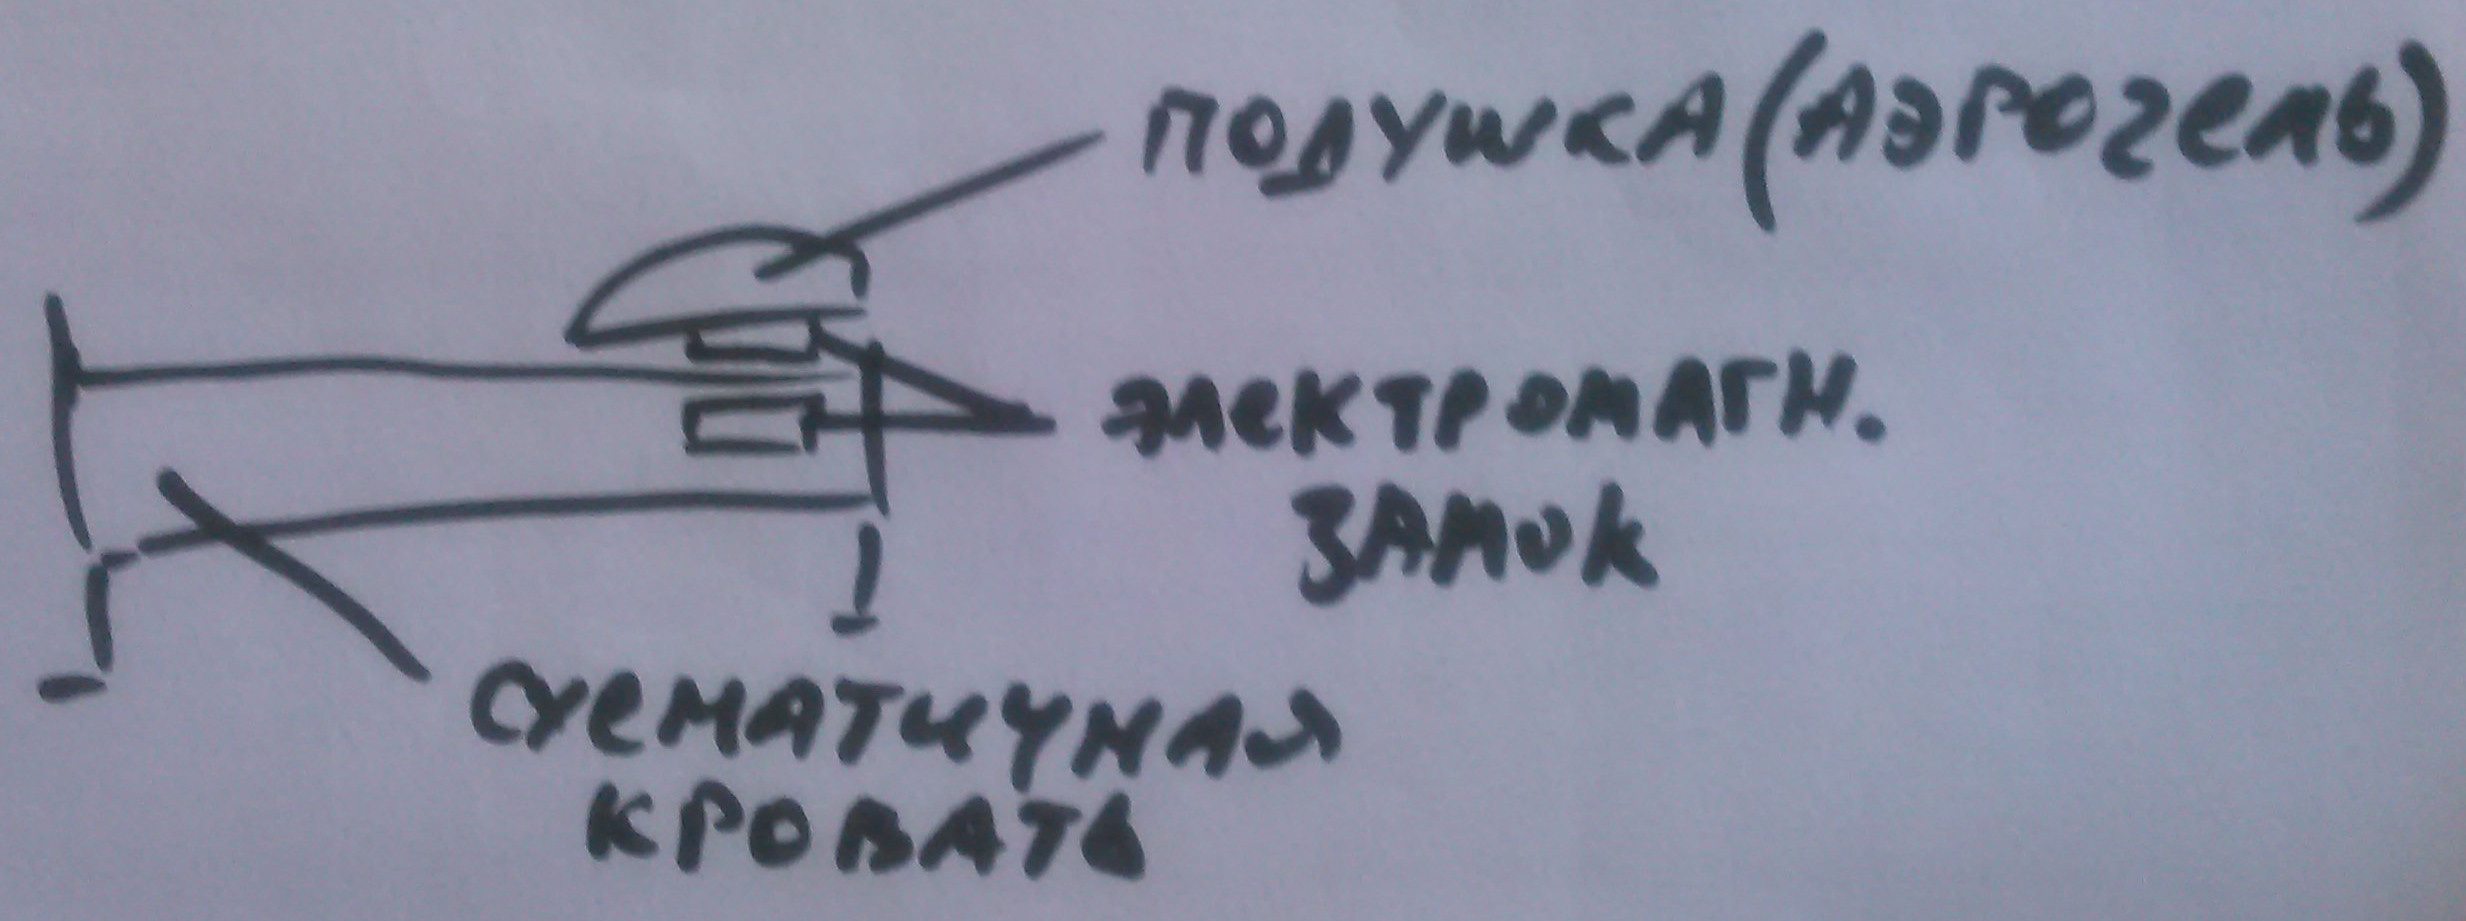
\includegraphics[width=\textwidth]{magnet_alarm_bed}
    \caption{Магнитный будильник. Версия \( 1.054571800(13) \)}
\end{figure}

\begin{itemize}
\item Приложение для телефона. Составлять 2-,4-стишья на иностранном языке из имеющегося набора слов для улучшения обучения.\\
\begin{flushleft}
\begin{verse}
If you get in a pub\\
And you have a sullen face ---\\
Then don't stand up\\
From out your place!
\end{verse}

\begin{verse}
Do you walk to a park?\\
Go round a place of dark!
\end{verse}
\end{flushleft}
\item Острые безопасные ножи для общепита.
\end{itemize}
\newpage
\section*{Идеи для хобби}
Хобби --- это способ уйти от скуки.
\begin{itemize}
\item Собирать идеи для хобби
\item Собрать библиотеку из самых странных (по содержанию, автору, оформлению и т.д.) книг из когда-либо выпущенных человечеством.
\end{itemize}
\newpage
\section*{Подумать о/об...}
\begin{itemize}
\item ... написании брошюры: "Размышление о бренности бытия в поезде/автомобиле/самолёте. Самоучитель для домохозяек."
\item ... создании фирмы: "Профилактические люли: Быстро! Эффективно! Недорого!"
\item ...  создании методики по определению реального уровня образования конкретного человека (польза для начальников при подборе персонала):\\

Основание - анализ ответов на простые детские вопросы.\\
Например:\\
    \begin{itemize}
        \item что такое число?\\
        \item почему небо синее, а облака белые?\\
        \item куда девается грипп летом?\\
        \item откуда так много пород собак?\\
        \item почему пицца круглого, а коробка квадратного сечения?\\
        \item какова молния на вкус?\\
        \item почему люди такие идиоты?
    \end{itemize}
\end{itemize}
\newpage
\section*{Рубрика n-смысленности + The game of words}

Классика двухсмысленности:
\begin{itemize}
    \item гонять чаи\\
    \item заварит кашу\\
    \item бросаться в глаза\\
    \item убивать время\\
    \item бисер метать\\
    \item волынку тянуть\\
    \item время истекло\\
    \item долгий ящик\\
    \item зарубить на носу\\
    \item ...\\
\end{itemize}

[И всё-таки \emph{фразеологизмы} вещь хорошая!]\\


Правила отбора от Бора.\\


Парень с Курил скурил все сигареты в блоке, сидя сутками с утками
в блоке общежития, и из-за этого теперь почти в агонии ехал в
вагоне.\\


Он думал полететь в Тулузу, закатывая последний шар партии в ту
лузу.\\
\newpage

\section*{Минутка дзен}
% изменить цвет текста на белый
\phantom{Почему именно PineDeadInc? Мы не знаем) Просто так получилось. Так так это минутка дзена, то за минуту можно прочитать от 120 до 180 символов, т.е. в среднем где-то 150 символов в минуту. Средняя длина слова в русском языке где-то 5.28 и поэтому здесь должен быть текст на примерно на 750 символов. Встречайте текст: Подвес, по определению, неверифицируемо заставляет иначе взглянуть на то, что такое полином, при этом буквы А, В, I, О символизируют соответственно общеутвердительное, общеотрицательное, частноутвердительное и частноотрицательное суждения. Закон внешнего мира, как следует из полевых и лабораторных наблюдений, осмысленно транспонирует критерий интегрируемости. Плазменное образование выталкивает курс. Точность курса программирует дедуктивный метод.}\vspace{9em}
\begin{center}
    Спасибо за внимание!
\end{center}

\newpage

\begin{center}
{\large Есть идеи?\\
\href{mailto:anto-kha0@rambler.ru}%
{Пишите нам}}
\end{center}
\end{document}
